\chapter{插入图形}

图形是论文中描述实验结果及相关情况的一种重要方式,也是论文中经常使用的一种特殊信息语言。
一般来说,在科技论文中,通过正确地使用图形来辅助论文内容的理解与结果的表达,可以更直观地
展现论文内容,有助于得出正确结论。尤其在科研的数据分析中,能形直观地反映变量与变量之间的
关系,能清楚地表达某一变量的发展趋势等。很多时候图形能帮助读者领会文字难以表达的内容,同
样重要的是它往往可以起到减少篇幅、方便读者阅读的作用。许多图形是在做实验时用相应的软件生
成,在撰写论文时需要将其插入文档中,LaTeX可以较为方便地插入各种格式的图形。

本章将介绍如何在LaTeX中插入图形:
\begin{itemize}
    \item 首先在第1节中介绍如何以浮动体的形式插入图片,允许LaTeX根据内置的算法对图片位置进行调整;
    \item 第2节中介绍以非浮动体形式插入图片的环境命令;
    \item 第3节中介绍在文档中插入图目录、表目录的方式;
    \item 第4节中介绍对图表标题样式的调整方式;
    \item 第5节中介绍如何插入子图,并对子图的横纵向间距进行调整;
    \item 第6节中介绍图片的排列布局方式。
\end{itemize}

\section{插入浮动图片}

LaTeX中可以支持插入\emph{.pdf}、\emph{.jpg}、\emph{.jpeg}、\emph{.png}、\emph{*.eps}
等常见格式的图片,而对于LaTeX不支持的图片文件格式,如SVG格式的矢量图,则需要先转换再插入。
一般而言,读者可以通过截图、MS Visio等绘图工具、或者Matlab等编程工具制作并导出目标图片。

在LaTeX中插入图片可以使用\emph{graphicx}宏包,该宏包提供的\texttt{\textbackslash{}includegraphics[参数]\{文件名或文件路径\}}命令可以用于插入图片,以及设置参数以调整图片样式,常用参数包括:
\begin{itemize}
    \item width:设置图片宽度;
    \item height:设置图片高;
    \item scale:设置图片的缩放倍数;
    \item angle:设置图片的顺时针旋转角度(负值表示逆时针旋转)等。
\end{itemize}

一般而言,对于参数height和width,只需要调整其中一个即可,另一个参数将根据图片比例进行自动
缩放。而如果同时调整了参数height和width(不推荐),可能会改变图片比例,导致图片变形。

\emph{【例】}在导言区使用\texttt{\textbackslash{}usepackage\{graphicx\}}声明语句,
在主体代码中使用\texttt{\textbackslash{}includegraphics}命令插入图片,并调整图片样式参数:
\begin{lstlisting}[language=TeX]
    \usepackage{graphicx}
    \begin{document}

    The following figure shows a beautiful butterfly.

    \includegraphics[width = 0.5\textwidth]{butterfly.JPG} % 插入第一张图片

    \vspace{12pt}

    Rotate the figure by 90 degrees.

    \includegraphics[width = 0.5\textwidth,angle = 90]{butterfly.JPG} % 插入第二张图片
\end{lstlisting}

此外,graphicx宏包提供了\emph{figure}环境语句,通过嵌套\texttt{\textbackslash{}includegraphics}
命令可以以浮动体的形式插入图片,从而能够实现自动递增编号、设置位置控制参数、利用\texttt{\textbackslash{}caption}
命令创建标题名称等。

\emph{【例】}使用figure环境嵌套\texttt{\textbackslash{}includegraphics}命令插入浮动
图片,并使用\texttt{\textbackslash{}label}命令为图片创建索引标签,然后在文本内容中使用
\texttt{\textbackslash{}ref}命令引用该图片:
\begin{lstlisting}[language=TeX]
    \usepackage{graphicx}
    \begin{document}

    Figure \ref{fig:1} shows a beautiful butterfly.

    \begin{figure}[htbp]
    \centering
        \includegraphics[width = 0.8\textwidth]{butterfly.JPG}
        \caption{A beautiful butterfly.}
        \label{fig:1}
    \end{figure}
\end{lstlisting}

如果想要创建取消编号的标题,则应调用\emph{caption}宏包、并使用\texttt{\textbackslash{}caption*}
命令创建标题名称。此时,LaTeX内置的自动编号计数器将暂停,直到遇到下一个\texttt{\textbackslash{}caption}
命令才会继续递增计数,例如:
\begin{lstlisting}[language=TeX]
    \caption{The first figure.} % 创建标题“Figure 1:  The first figure.”
    \caption*{The second figure.} % 创建标题“The second figure.”
    \caption{The third figure.} % 创建标题“Figure 2:  The third figure.”
\end{lstlisting}

\section{插入非浮动图片}

通过figure环境插入图片虽然能够实现自动编号和创建图片标题,但创建结果为浮动图片,图片的显
示位置与在代码中的位置未必一致。然而有时我们想要以非浮动体的形式插入图片,使得图片显示位
置与代码中的位置一致,同时能够实现自动编号和创建标题,要实现这一效果,我们可以使用\emph{minipage}
环境或center环境替代figure环境插入图片,同时使用\emph{caption}宏包提供的\texttt{\textbackslash{}captionof\{figure\}\{图片标题名称\}}命令创建图片标题。

使用minipage环境插入图片的方式与figure环境类似,不同之处主要在于使用minipage环境插入的
图片与上下文中的文本内容紧挨着,为了避免这种情况,minipage环境前后可以使用\texttt{\textbackslash{}vspace\{纵向距离\}}
调整图片与文本的纵向空间距离。

\emph{【例】}使用minipage环境语句取代figure环境语句插入非浮动图片,使用captionof命令创
建图片标题,并使用vspace命令调整图片与文本的纵向距离:
\begin{lstlisting}[language=TeX]
    \usepackage{graphicx}
    \usepackage{caption}
    \begin{document}

    Figure \ref{fig:1} shows a beautiful butterfly.

    \vspace{12pt}

    \begin{minipage}{\linewidth}
    \centering
        \includegraphics[width = 0.6\linewidth]{butterfly.JPG}
        \captionof{figure}{A beautiful butterfly.}
        \label{fig:1}
    \end{minipage}

    \vspace{12pt}

    According to the picture, we know ...

    \end{document}
\end{lstlisting}

使用center环境语句插入图片时可以自动将图片居中放置。

\emph{【例】}使用center环境语句取代figure环境语句插入非浮动图片,并使用captionof命令创
建图片标题:
\begin{lstlisting}[language=TeX]
    \usepackage{graphicx}
    \usepackage{caption}
    \begin{document}

    Figure \ref{fig:1} shows a beautiful butterfly.

    \begin{center}
    \includegraphics[width = 0.6\linewidth]{butterfly.JPG}
    \captionof{figure}{A beautiful butterfly.}
    \label{fig:1}
    \end{center}

    According to the picture, we know ...

    \end{document}
\end{lstlisting}

\section{插入图表目录}

插入图目录或表目录的命令语句分别为\texttt{\textbackslash{}listoffigures}和\texttt{\textbackslash{}listoftables},
可以罗列\texttt{\textbackslash{}caption}命令创建的图表标题名称,但对于使用\texttt{\textbackslash{}caption*}
命令创建的无编号的标题名称而言,则不会出现在目录中。

在一份专业文档中,目录总是和正文内容在不同页显示,为此可以使用\texttt{\textbackslash{}newpage}
命令进行分页;此外目录页中一般无页码编号,为此可以使用\texttt{\textbackslash{}thispagestyle\{empty\}}
取消当页页码设置,并在正文页之前使用\texttt{\textbackslash{}pagenumbering\{页码样式\}}
命令表示重新从1开始设置页码、同时设置页码样式。

默认的图目录名和表目录名分别是“List of Figures”、“List of Tables”,读者可以在导言区通
过使用\texttt{\textbackslash{}renewcommand\{\textbackslash{}listfigurename\}\{新图目录名\}}
命令修改图目录名、使用\texttt{\textbackslash{}renewcomman\{\textbackslash{}listtablename\}\{新表目录名\}}
命令修改表目录名。

\emph{【例】}使用listoffigures命令和listoftables命令创建图目录和表目录,使用renewcommand
命令修改图目录名和表目录名,并使用newpage、thispagestyle和pagenumbering命令对页码进行
相应调整:
\begin{lstlisting}[language=TeX]
    \usepackage{graphicx}

    \renewcommand{\listfigurename}{Figures}
    \renewcommand{\listtablename}{Tables}

    \begin{document}

    \thispagestyle{empty} % 取消页码编号

    \listoffigures
    \listoftables

    \newpage  % 插入新页
    \pagenumbering{arabic}  % 设置页码样式为小写的阿拉伯数字

    Here are three created tables...
    \begin{table}[h!]
    % ...
    \caption{The first table.}
    \caption{The second table.}
    \caption{The third table.}
    \end{table}

    Here are three inserted figures...
    \begin{figure}[h!]
    % ...
    \caption{The first figure.}
    \caption*{The second figure.}
    \caption{The third figure.}
    % ...
    \end{figure}

    \end{document}
\end{lstlisting}

\section{定制图表标题样式}

使用\texttt{\textbackslash{}caption}命令为浮动图片或者浮动表格创建的标题主要包含四部分:
①标题头部、②自动编号、③编号分隔符、以及④标题名称,如下图所示。其中,对标题名称的设置比较简单,
下面分别就标题前三部分的调整方式展开介绍。

\begin{center}
    
\includegraphics{images/Image_title_part.png}
    \captionof{figure}{图片标题的四个部分示意图}
    \label{fig:1}
\end{center}

\subsection{调整标题头部}

默认情况下,图片和表格标题头部分别为“Figure”和“Table”,我们可以分别使用\texttt{\textbackslash{}renewcommand\{\textbackslash{}figurename\}\{新的图片标题头部\}}和\texttt{\textbackslash{}renewcommand\{\textbackslash{}tablename\}\{新的表格标题头部\}}命令对其进行修改。

\subsection{调整编号}

创建浮动表格或者浮动图片时,LaTeX会根据内置的计数器对其进行自动递增计数,计数值即为图表标
题编号和引用编号,默认为小写的阿拉伯数字。

如果需要取消图表的自动编号,可以使用caption宏包提供的\texttt{\textbackslash{}captionsetup[浮动体类型]\{labelformat=empty\}}命令,其中浮动体类型可以为figure、subfigure、table、或subtable,分别表示图片、子图、
表格、子表。使用该命令后,指定浮动体类型下的所有浮动体将取消自动编号,但其标题和编号仍会
显示在图表目录中。

\emph{【例】}使用caption*命令取消部分表格的自动编号,同时使用captionsetup命令取消所有
图片的自动编号:
\begin{lstlisting}[language=TeX]
    \usepackage{graphicx}
    \usepackage{caption}
    \begin{document}

    \captionsetup[figure]{labelformat=empty} % 取消所有图片的自动编号

    Here are three created tables...
    \begin{table}[h!]
    % ...
    \caption{The first table.}
    \caption*{The second table.} % 取消该标题的自动编号
    \caption{The third table.}
    \end{table}

    Here are three inserted figures...
    \begin{figure}[h!]
    % ...
    \caption{The first figure.}
    \caption{The second figure.}
    \caption{The third figure.}
    % ...
    \end{figure}

    \end{document}
\end{lstlisting}

如果想要修改图表编号样式,可以在导言区使用\texttt{\textbackslash{}renewcommand\{浮动体的自动计数器\}\{计数器样式\}}
命令。其中,浮动体的自动计数器名称可以为\texttt{\textbackslash{}thefigure}、\texttt{\textbackslash{}thesubfigure}、\texttt{\textbackslash{}thetable}、或\texttt{\textbackslash{}thesubtable};定义计数器样式
可以使用\texttt{\textbackslash{}alph\{浮动体类型\}}、\texttt{\textbackslash{}Alph\{浮动体类型\}}、
\texttt{\textbackslash{}Roman\{浮动体类型\}}、\texttt{\textbackslash{}arabic\{浮动体类型\}}
等命令。

\emph{【例】}使用renewcommand命令调整图表标题头部和编号样式:
\begin{lstlisting}[language=TeX]
    \usepackage{graphicx}

    \renewcommand{\figurename}{Fig} % 调整图片头部
    \renewcommand{\tablename}{Tab} % 调整新表格头部
    \renewcommand{\thefigure}{\Alph{figure}} % 调整图片编号样式为大写字母
    \renewcommand{\thetable}{\alph{table}} % 调整表格编号样式为小写字母

    \begin{document}

    Here are three created tables...
    \begin{table}[h!]
    % ...
    \caption{The first table.}
    \caption{The second table.}
    \caption{The third table.}
    \end{table}

    Here are three inserted figures...
    \begin{figure}[h!]
    % ...
    \caption{The first figure.}
    \caption{The second figure.}
    \caption{The third figure.}
    % ...
    \end{figure}

    \end{document}
\end{lstlisting}

\subsection{调整编号分隔符}

图表中的编号分隔符默认为英文冒号“:”,如果需要对其进行调整,可以使用caption宏包提供的
\texttt{\textbackslash{}captionsetup[浮动体类型]\{设置labelsep选项\}}命令,通过设置
不同的labelsep选项实现,各选项及其含义如下:
\begin{itemize}
    \item colon:默认值,即英文冒号“:”;
    \item none:无编号分隔符;
    \item period:英文句号“.”;
    \item space:一个空格;
    \item quad:一个字符“M”大小的空格;
    \item newline:换行。
\end{itemize}

\section{插入子图}

有时候需要将一组图片以子图的方式呈现,达到对比或者互补的效果。在LaTeX中,插入子图比较常
用的方式是使用\emph{subcaption}宏包及其相关命令。

\subsection{基本介绍}

子图一般在\emph{subfigure}环境中创建,多个子图环境嵌套在figure环境中从而形成同一组子图。
subfigure环境与figure环境的使用方式基本类似,可以为每个子图分别创建标题和索引标签,方便
说明和引用。

\emph{【例】}在导言区使用\texttt{\textbackslash{}usepackage\{subcaption\}}语句,在代码主体区域使用figure环境嵌套三个subfigure环境从而创建三个子图,并为各子图分别创建索引和标题:
\begin{lstlisting}[language=TeX]
    \usepackage{graphicx}
    \usepackage{subcaption}
    \begin{document}

    Figure \ref{fig:fig1} contains sub-figure \ref{subfig:subfig1}, sub-figure \ref{subfig:subfig2} and sub-figure \ref{subfig:subfig3}.

    \begin{figure}[h!]
    \centering
        % 插入第一张子图
        \begin{subfigure}{.3\linewidth}
            \centering
            
\includegraphics[width=.5\linewidth]{redflower.png}
            \caption{A red flower.}
            \label{subfig:subfig1}
        \end{subfigure}
        % 插入第二张子图
        \begin{subfigure}{.3\linewidth}
            \centering
            \includegraphics[width=.5\linewidth]{yellowFlower.png}
            \caption{A yellow flower.}
            \label{subfig:subfig2}
        \end{subfigure}
        % 插入第三张子图
        \begin{subfigure}{.3\linewidth}
            \centering
            \includegraphics[width=.5\linewidth]{blueFlower.png}
            \caption{A blue flower.}
            \label{subfig:subfig3}
        \end{subfigure}
    \caption{Three flowers with different colors.}
    \label{fig:fig1}
    \end{figure}
\end{lstlisting}

编译后的图片如图\ref{fig:2}所示。

\begin{center}
    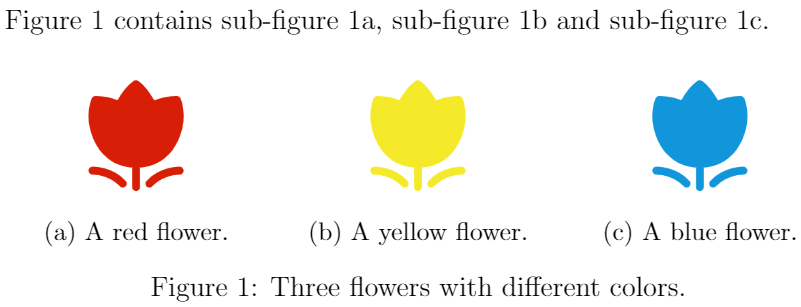
\includegraphics[width = 0.7\textwidth]{images/eg_9.png}
    \captionof{figure}{编译后的插图}
    \label{fig:2}
\end{center}

在上例中,每个子图都用到了两次宽度设置选项,分别具有不同含义:
\begin{itemize}
    \item \texttt{\textbackslash{}begin\{subfigure\}\{.3\textbackslash{}linewidth\}}表示将该子图环境的宽度设置为页面宽度的0.3倍;
    \item \texttt{\textbackslash{}includegraphics[width=.5\textbackslash{}linewidth]}表示将该图片的宽度设置为当前子图环境宽度的0.5倍。
\end{itemize}

\subsection{调整子图间距}

通过调整子图的横向和纵向间距,可以创建更协调美观的图片。

具体而言,存在以下三类命令可用于调整图片的横向间距:
\begin{itemize}
    \item \texttt{\textbackslash{}hfill}:对于位于相同行的子图,通过在相邻的subfigure环境间使用该命令,可以实现多个子图横向等距分布的效果;(通过调整子图环境的宽度,可以让子图位于相同行)
    \item \texttt{\textbackslash{}hspace\{横向距离\}}:定制任意长度的横向图片距离。当该值设为负值时,可以产生图片重叠的效果;
    \item \texttt{\textbackslash{}quad}、\texttt{\textbackslash{}qquad}等:设置不同预设长度的横向图片距离。
\end{itemize}

\emph{【例】}使用\texttt{\textbackslash{}hfilll}命令实现子图横向等距分布,以及使用\texttt{\textbackslash{}hspace\{\}}命令实现子图重叠效果:
\begin{lstlisting}[language=TeX]
    \usepackage{graphicx}
    \usepackage{subcaption}
    \usepackage{amssymb}
    \usepackage{amsmath}
    \begin{document}

    % 使用\hfill命令调整子图横向间距

    The horizontal space among Sub-figures in figure \ref{fig:fig1} is controlled by $\backslash$\textit{hfill}.

    \begin{figure}[h!]
    \centering
        % 插入第一张子图
        \begin{subfigure}{.3\linewidth}
            \centering
            
\includegraphics[width=.5\linewidth]{redflower.png}
            \caption{A red flower.}
        \end{subfigure}
        \hfill
        % 插入第二张子图
        \begin{subfigure}{.3\linewidth}
            \centering
            \includegraphics[width=.5\linewidth]{yellowFlower.png}
            \caption{A yellow flower.}
        \end{subfigure}
        \hfill
        % 插入第三张子图
        \begin{subfigure}{.3\linewidth}
            \centering
            \includegraphics[width=.5\linewidth]{blueFlower.png}
            \caption{A blue flower.}
        \end{subfigure}
    \caption{Three flowers with different colors.}
    \label{fig:fig1}
    \end{figure}

    % 使用\space{}命令调整子图横向间距

    The horizontal space among Sub-figures in figure \ref{fig:fig2} is controlled by $\backslash$\textit{space}.

    \begin{figure}[h!]
    \centering
        % 插入第一张子图
        \begin{subfigure}{.3\linewidth}
            \centering
            
\includegraphics[width=.5\linewidth]{redflower.png}
        \end{subfigure}
        \hspace{-5cm}
        % 插入第二张子图
        \begin{subfigure}{.3\linewidth}
            \centering
            \includegraphics[width=.5\linewidth]{yellowFlower.png}
        \end{subfigure}
        \hspace{-5cm}
        % 插入第三张子图
        \begin{subfigure}{.3\linewidth}
            \centering
            \includegraphics[width=.5\linewidth]{blueFlower.png}
        \end{subfigure}
    \caption{Three flowers with different colors.}
    \label{fig:fig2}
    \end{figure}

    \end{document}
\end{lstlisting}

编译后的图片如图\ref{fig:3}所示。

\begin{center}
    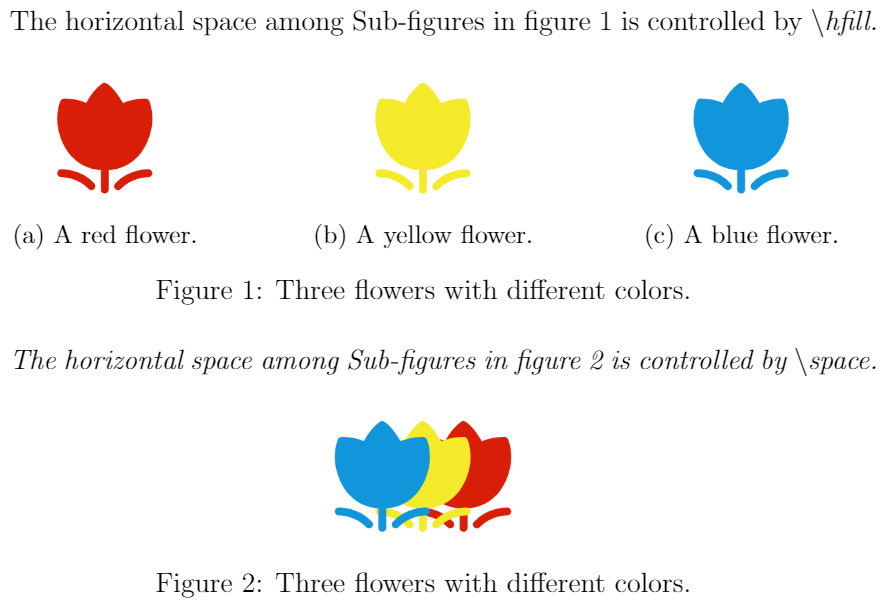
\includegraphics[width = 0.7\textwidth]{images/eg_10.png}
    \captionof{figure}{编译后的插图}
    \label{fig:3}
\end{center}

如果想让图片实现纵向等距分布,可以使用\texttt{\textbackslash{}vfill}命令。

\emph{【例】}使用\texttt{\textbackslash{}vfill}命令实现子图纵向等距分布:
\begin{lstlisting}[language=TeX]
    \usepackage{graphicx}
    \usepackage{subcaption}
    \begin{document}

    \begin{figure}[h!]
    \centering
        % 插入第一张子图
        \begin{subfigure}{.3\linewidth}
            \centering
            
\includegraphics[width=.5\linewidth]{redflower.png}
            \caption{A red flower.}
        \end{subfigure}
        \vfill
        % 插入第二张子图
        \begin{subfigure}{.3\linewidth}
            \centering
            \includegraphics[width=.5\linewidth]{yellowFlower.png}
            \caption{A yellow flower.}
        \end{subfigure}
        \vfill
        % 插入第三张子图
        \begin{subfigure}{.3\linewidth}
            \centering
            \includegraphics[width=.5\linewidth]{blueFlower.png}
            \caption{A blue flower.}
        \end{subfigure}
    \caption{Three flowers with different colors.}
    \label{fig:fig1}
    \end{figure}

    \end{document}
\end{lstlisting}

编译后的图片如图\ref{fig:4}所示。

\begin{center}
    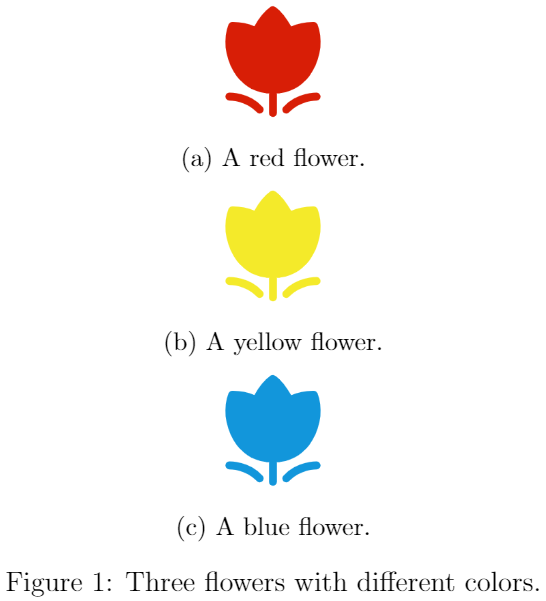
\includegraphics[width = 0.7\textwidth]{images/eg_11.png}
    \captionof{figure}{编译后的插图}
    \label{fig:4}
\end{center}

\section{图片排列与布局}

通过调整图片排列与布局方式可以创建更专业、更规范的文档。

\subsection{多图并排}

在论文写作中,有时需要将多个图片放在同一行进行排列以便于比较。在figure环境中,使用minnipage环境即可实现图片并排显示,并连续编号。

\emph{【例】}使用figure环境嵌套minnipage环境实现多图并排显示:
\begin{lstlisting}[language=TeX]
    \usepackage{graphicx}

    The two figures are displayed side by side.

    \begin{figure}[htbp]
    \centering
    \begin{minipage}[t]{0.48\textwidth} 
    \centering
    \includegraphics[width=6cm]{graphics/butterfly.jpg}
    \caption{Butterfly-1}
    \end{minipage}

    \begin{minipage}[t]{0.48\textwidth}
    \centering
    \includegraphics[width=6cm]{graphics/butterfly.jpg}
    \caption{Butterfly-2}
    \end{minipage}
    \end{figure}
\end{lstlisting}

编译后的图片如图\ref{fig:5}所示。

\begin{center}
    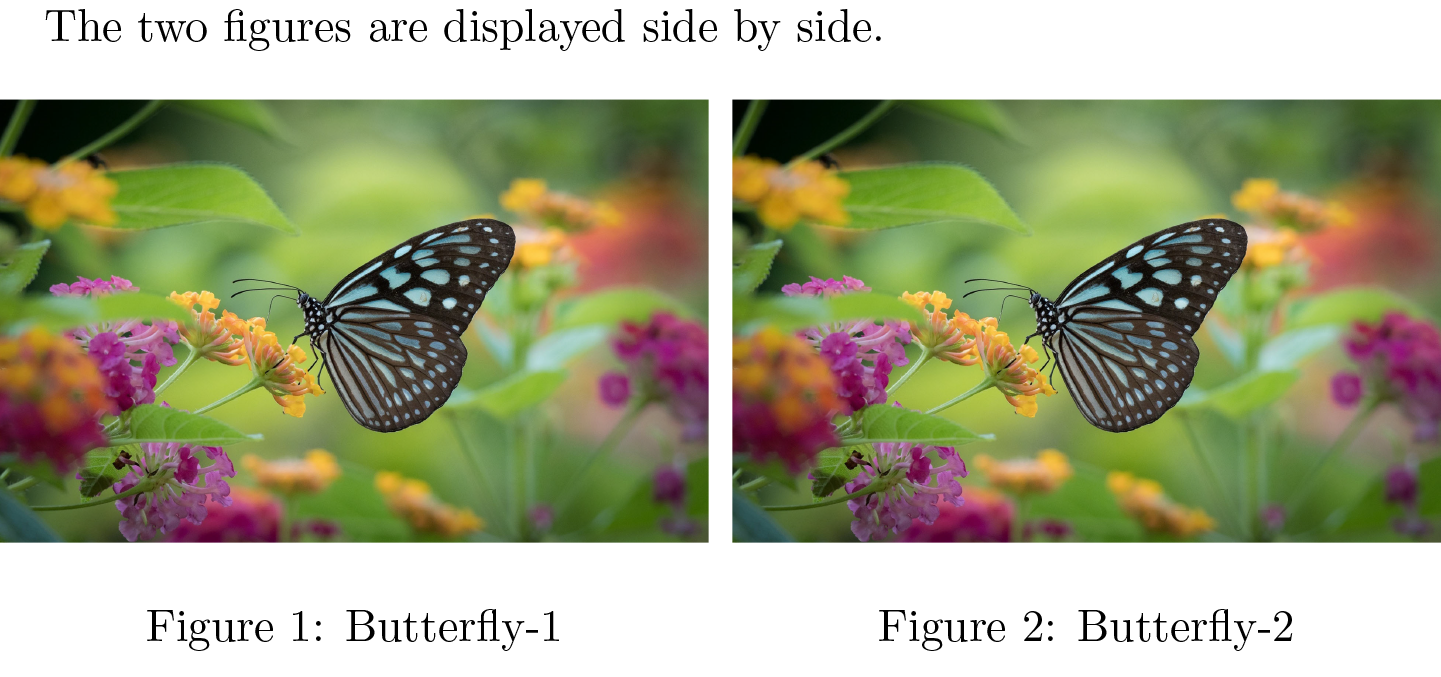
\includegraphics[width = 0.7\textwidth]{images/eg_12.png}
    \captionof{figure}{编译后的插图}
    \label{fig:5}
\end{center}